\section{Application to protoplanetary disks}\label{2dppd}
We now apply our linear framework to assess the stability of realistic 
protoplanetary disks. We consider the gravito-turbulent disk models recently
developed by \cite[][hereafter \citetalias{rafikov15}]{rafikov15}. 
This 2D, Keplerian disk orbits a Solar 
mass star and is defined by the following parameters, 

\begin{itemize}
  \item $\dot{M}$, the global radial mass accretion rate;
  \item $Q_0$, the value of the 2D Toomre parameter where the disk is
    gravito-turbulent;
  \item $T_\mathrm{irr}$, the irradiation or floor temperature;
  \item $\alpha_m$, the dimensionless viscosity associated with other
    sources of turbulence, such as magneto-rotational instabilities
    (MRI), see also \S\ref{visc_gi} and \S\ref{MHD}. 
\end{itemize} 
These are used in the statements of thermal equilibrium, mass and
angular momentum conservation, together with an opacity law, 
to construct a global disk model with surface density $\Sigma(R)$ and
temperature $T(R)$ where $R$ is the global cylindrical radius from the
star. \citepalias[See][for details.]{rafikov15} This gives the $Q(R)$
value required for input into our linear framework. We derive other
dimensionless parameters below. 

Note that we are considering the local stability at each radius. We
are thus neglecting the slow, background viscous radial flow; as well
as any global gravitational instabilities \citep{lodato05}. {\bf more refs?}

\subsection{Effective $\alpha$}
In a steady, viscously accreting Keplerian disk 
with constant $\dot{M}$ we have,
approximately, $\nu\Sigma = \dot{M}/3\pi$. Hence
\begin{align}
  \alpha = \frac{\dot{M}}{3\pi}\frac{\Omega(R)}{c_{s}^2(T)\Sigma(R)},  
\end{align} 
which sets the viscosity coefficient to be used at each radius. 

\subsection{PPD beta cooling}
Energy loss in \citetalias{rafikov15} is given by 
\begin{align}\label{real_cool}
  \Lambda = \frac{2\sigma}{f(\tau)}\left(T^4 - T_\mathrm{irr}^4\right)
\end{align}
per unit area, 
\begin{align}
  f(\tau) = \tau + \frac{1}{\tau}, \label{ftau} 
\end{align}
and
\begin{align}
  \tau = \kappa_d(T)\Sigma
\end{align}
is the optical depth and recall Eq. \ref{opacity_law} 
is our opacity model where $\kappa_d\propto T^b$ with $b=2$. 
Eq. \ref{ftau} accounts for cooling in the optically-thin ($\tau\ll
1$) and optically-thick ($\tau\gg1$) regimes. 

Note that Eq. \ref{real_cool} is a beta cooling prescription because
it is an explicit function of the thermodynamic states. However, we
formulated the linear problem with beta cooling of the functional form
given by Eq. \ref{beta_cool}. In order to adapt the developed
framework to the above PPD beta cooling function, we
need to identify the $\beta$ and $\theta$ parameters that enter the 
linearized equations (Eq. \ref{linear_beta}). 
 
%Since we are interested in the linear response of the system, the
%corresponding cooling parameters $\beta$ and $\theta$ are found by
%comparing the linearized form of the cooling function
%(Eq. \ref{real_cool}) to that of the model function
%(Eq. \ref{beta_cool}).  

%{\bf as opposed to comparing their unperturbed forms, as done in literature}
Linearizing Eq. \ref{real_cool} gives   
\begin{align}\label{linear_real_cool}
  (\gamma-1)\frac{\delta\Lambda}{\Sigma} = \frac{2\sigma(\gamma-1)
    T^4C_1}{f(\tau)c_{s}^2\Sigma}\left(\frac{\delta P}{\Sigma} -
  \frac{C_2}{C_1}c_{s}^2\frac{\delta\Sigma}{\Sigma}\right), 
\end{align}
where
\begin{align}
C_1(\tau, T) &= 4 - b\times g(\tau, T),\\ 
C_2(\tau, T) &= 4 + (1-b)\times g(\tau, T),\\ 
  g(\tau, T) &= \left( \frac{\tau^2-1}{\tau^2+1}\right)\left(1 -
  \frac{T_\mathrm{irr}^4}{T^4}\right). \label{g_def}
\end{align}
Comparing Eq. \ref{linear_real_cool} with the linearized form of the
standard cooling function, Eq. \ref{linear_beta}, we identify
\begin{align}
  &\beta = \frac{f(\tau)c_s^2\Sigma\Omega}{2\sigma(\gamma-1)C_1T^4},\label{real_beta}\\
  &\theta = \frac{C_2}{C_1},\label{real_theta} 
\end{align}
to be used in the 2D dispersion relation (Eq. \ref{thindisk}). 

Eq. \ref{real_beta} still represents a physical (dimensionless) cooling
time, and is consistent with previous definitions of realistic cooling
times within factors of order unity \citep[e.g.][their
Eq. 2]{kratter10}.  

However, $\theta$ is now an effective 
irradiation level. 
%no longer a direct measure of
%irradiation. 
Eq. \ref{real_theta} shows that $\theta$ is related to the true
irradation temperature $\tirr$ through the function $g$ given by 
Eq. \ref{g_def}. This is
important because a physically non-irradiated disk with $\tirr=0$ will
still have a non-zero effective irradiation, $\theta\neq0$. 
%This results from the fact that PPD cooling generally depends on both
%$P$ and $\Sigma$, but in the absence of irradiation standard beta
%cooling only depends on $P$. 

%On the
%other hand, fully irradiated disks with  $T=T_\mathrm{irr}$ have 
%$\theta=1$, as is in the previous problem formulation
%(Eq. \ref{tirr_def}). 

%the gammie-type cooling function does not represent realistic
%cooling. because real cooling depends on sigma and pressure but gammie
%cooling only depends on pressure 

\subsection{Inviscid stability condition}
We note that for our adopted opacity law, Eq. \ref{opacity_law}, 
\begin{align*}
  \theta = \frac{4-g}{4-2g},
\end{align*}
implying $5/6<\theta<3/2$. 
From the discussion in \S\ref{2d_inviscid} and applying
Eq. \ref{stable_condition},  we conclude that without viscous effects 
the disk is stable everywhere if  
\begin{align} 
  \gamma > \frac{3}{2} \quad \text{and} \quad Q >
  \sqrt{\frac{6}{5}} \label{ppd_invisc_cond} 
\end{align} 
are both satisfied.  

PPDs become irradiation-dominated at large distances from the star,
where $T\to\tirr$, or $\theta\to 1$. {\bf ref?}
Then the first inequality in Eq. \ref{ppd_invisc_cond} relaxes to
$\gamma > 1$ in the outer disk, which is always satisfied.  
On the other hand, numerical simulations of gravito-turbulence
show that $1\lesssim Q \lesssim 2$ \citep{gammie01,rice11}, and 
the second inequality is generally satisfied. Taken together, this
means that in the outer regions of a realistic PPD, cooling itself
cannot cause instability.  

\subsection{Example 2D calculation}\label{pp2d_example}
We consider a model with $\dot{M} = 10^{-6}M_\sun\,\yr^{-1}$, $Q_0=1.5$, 
$\tirr=10\mathrm{K}$, and $\alpha_m=10^{-3}$. 
We adopt the opacity scale $\kappa_{d0} =
5\times10^{-4}\mathrm{cm}^2\,\mathrm{g}^{-1}\,\mathrm{K}^{-2}$  as in
\citetalias{rafikov15}. We use $\gamma=1.6$, approximately applicable
to molecular gas at low temperatures and used by other authors
\citep{rice11,baehr15}. Then the global inviscid stability condition
(Eq. \ref{ppd_invisc_cond}) is satisfied. 
%for outer disk choice of gamma doesn't matter 
%avoid complications from over-stable thermal modes 
Fig. \ref{rafikov_model} shows the equilirbium 
disk profile in terms of $Q$, $\alpha$, $\beta$, and $\theta$.  
These are set as input to the 2D dispersion relation
(Eq. \ref{thindisk}).    

Fig. \ref{rafikov_growth} show growth timescales and
optimum wavenumbers for viscous GI in this disk model.  
We also plot analytic estimates based on Eq. \ref{gammie_smallk} (instead of
Eq. \ref{gammie_maxrate_simple} since here $\theta\sim 1$) 
which gives the optimum wavenumber as
\begin{align}
  |K| = \frac{3}{2\theta Q},
\end{align}
with growth rate
\begin{align} 
  S = \frac{27\alpha}{16\theta^3Q^4}. 
\end{align}
These are similar to the isothermal results of
\citet[][their Eq. 19 and 21, respectively]{sterzik95}, and identical if one
takes $\theta=1$. %showing that irradiation makes the disk behave like
                  %isothermal disk
 
The most unstable wavelength is a few times the disk thickness. The
increase in $|K|$ from $\sim 10\mathrm{AU}$ to $\sim 20\mathrm{AU}$ is
due to the decrease in $Q$; while that from $\sim 60\mathrm{AU}$ to
$\sim 100\mathrm{AU}$ occurs as the disk transitions from
optically-thick to optically-thin regimes. The mismatch at large
distances is  
not surprising since the above expressions assume $|K|\ll
1$. Nevertheless the analytic estimates reproduce the correct
behavior.  

The disk is subject to viscous GI on dynamical timescales ($\lesssim
10$ orbits) for $R\gtrsim60$AU. Coincidentally, beyond this radius
$\alpha\gtrsim 0.1$ and $\beta\lesssim 3$, which is often quoted as 
criteria for disk fragmentation \citep[e.g.][]{rafikov15}. 
This suggests that fragmentation in the outer parts of a realistic PPD
occurs is physically due to large turbulent stresses. 

%{\bf despite apply beta cooling results to realistic cooling disks}
%Our result suggest an alternative interpretation of disk fragmentation
%is where the gravito-turbulent state becomes dynamically unstable due to
%both viscosity and self-gravity. 
%{\bf note: disk might be stablized by extremely large alpha at large
%  distances but `turbulent' framework no longer valid }

\begin{figure}
  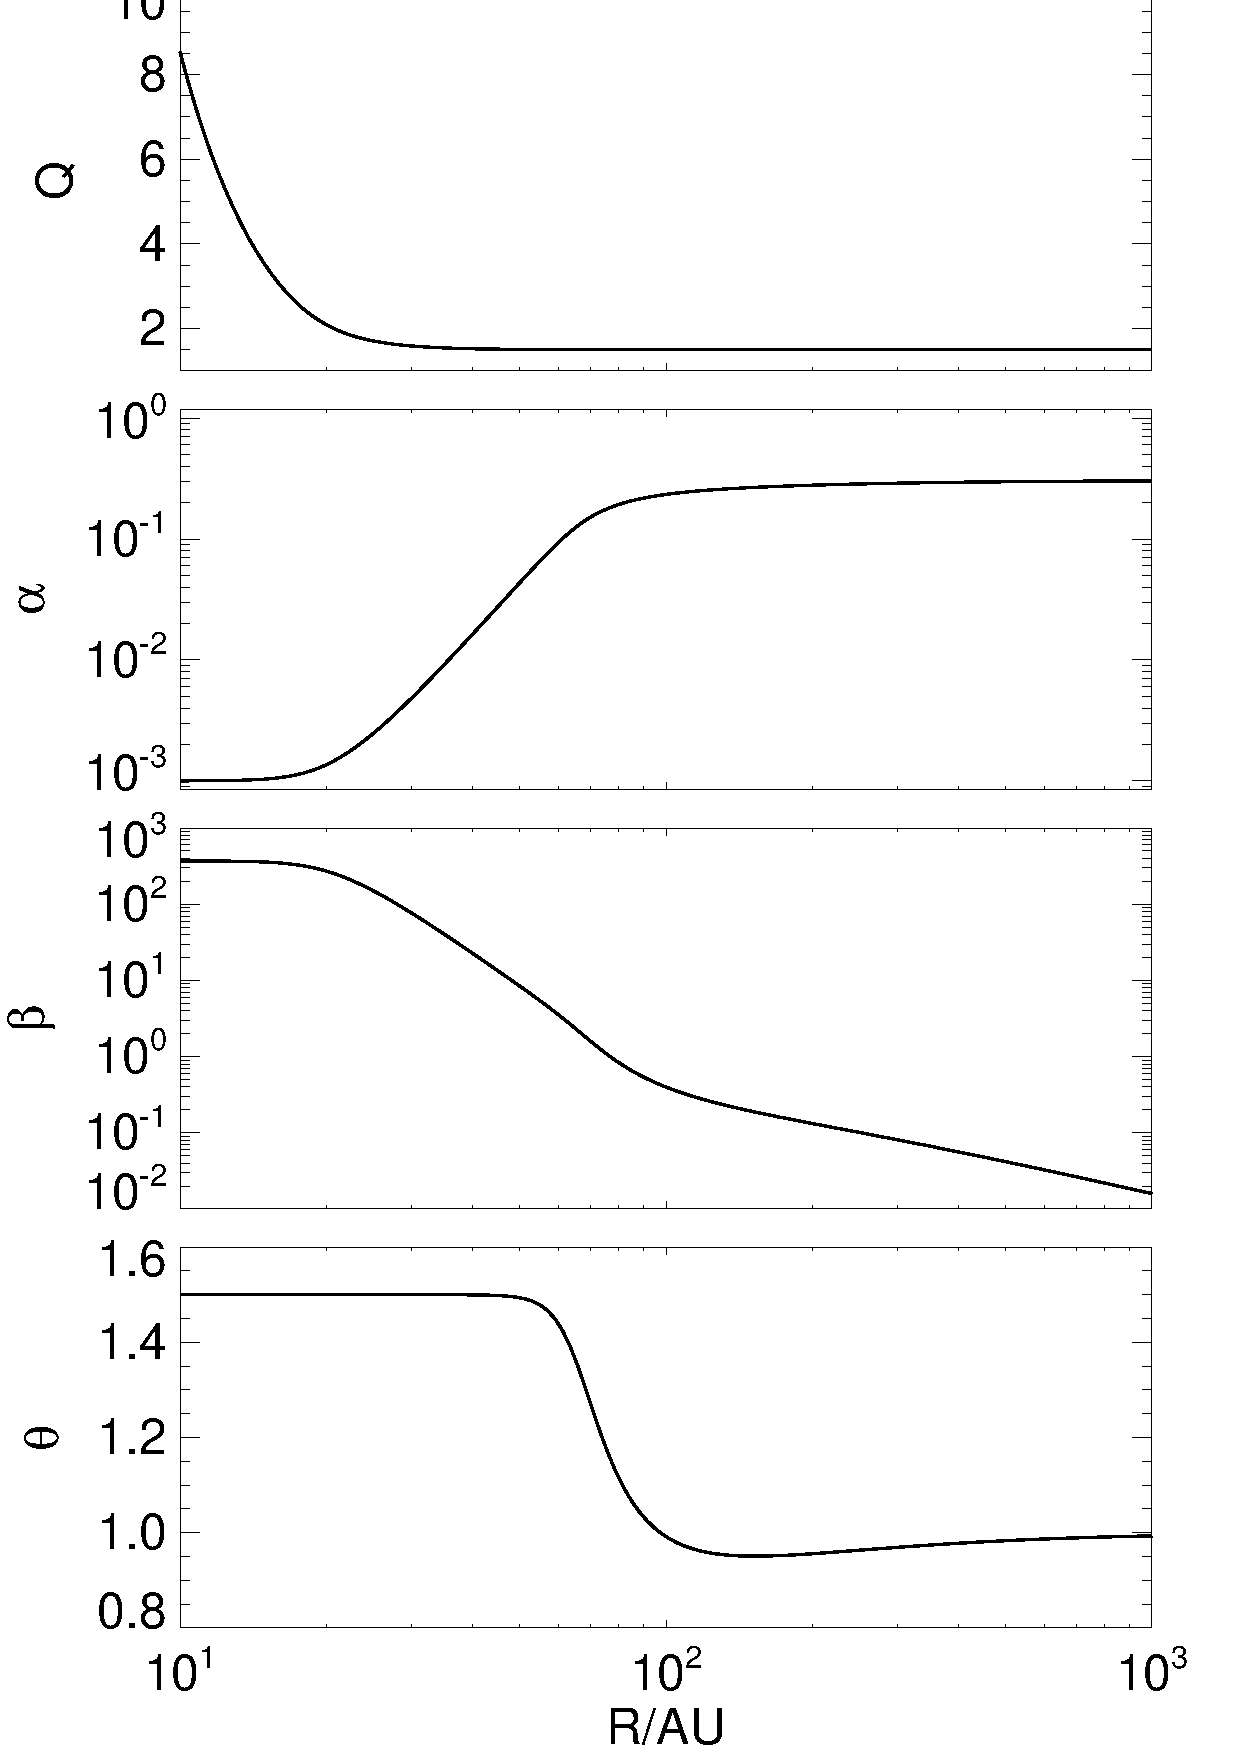
\includegraphics[width=\linewidth,clip=true,trim=0cm 0cm 0cm
    0.0cm]{figures/ppd_2d_basic}
  \caption{Equilibrium profile obtained from the disk model developed
    by \cite{rafikov15}, with parameters $\dot{M} =
    10^{-6}M_\sun\yr^{-1}$, $Q_0=1.5$, $\tirr=10\mathrm{K}$, and
    $\alpha_m=10^{-3}$.   
    \label{rafikov_model}}
\end{figure}

\begin{figure}
  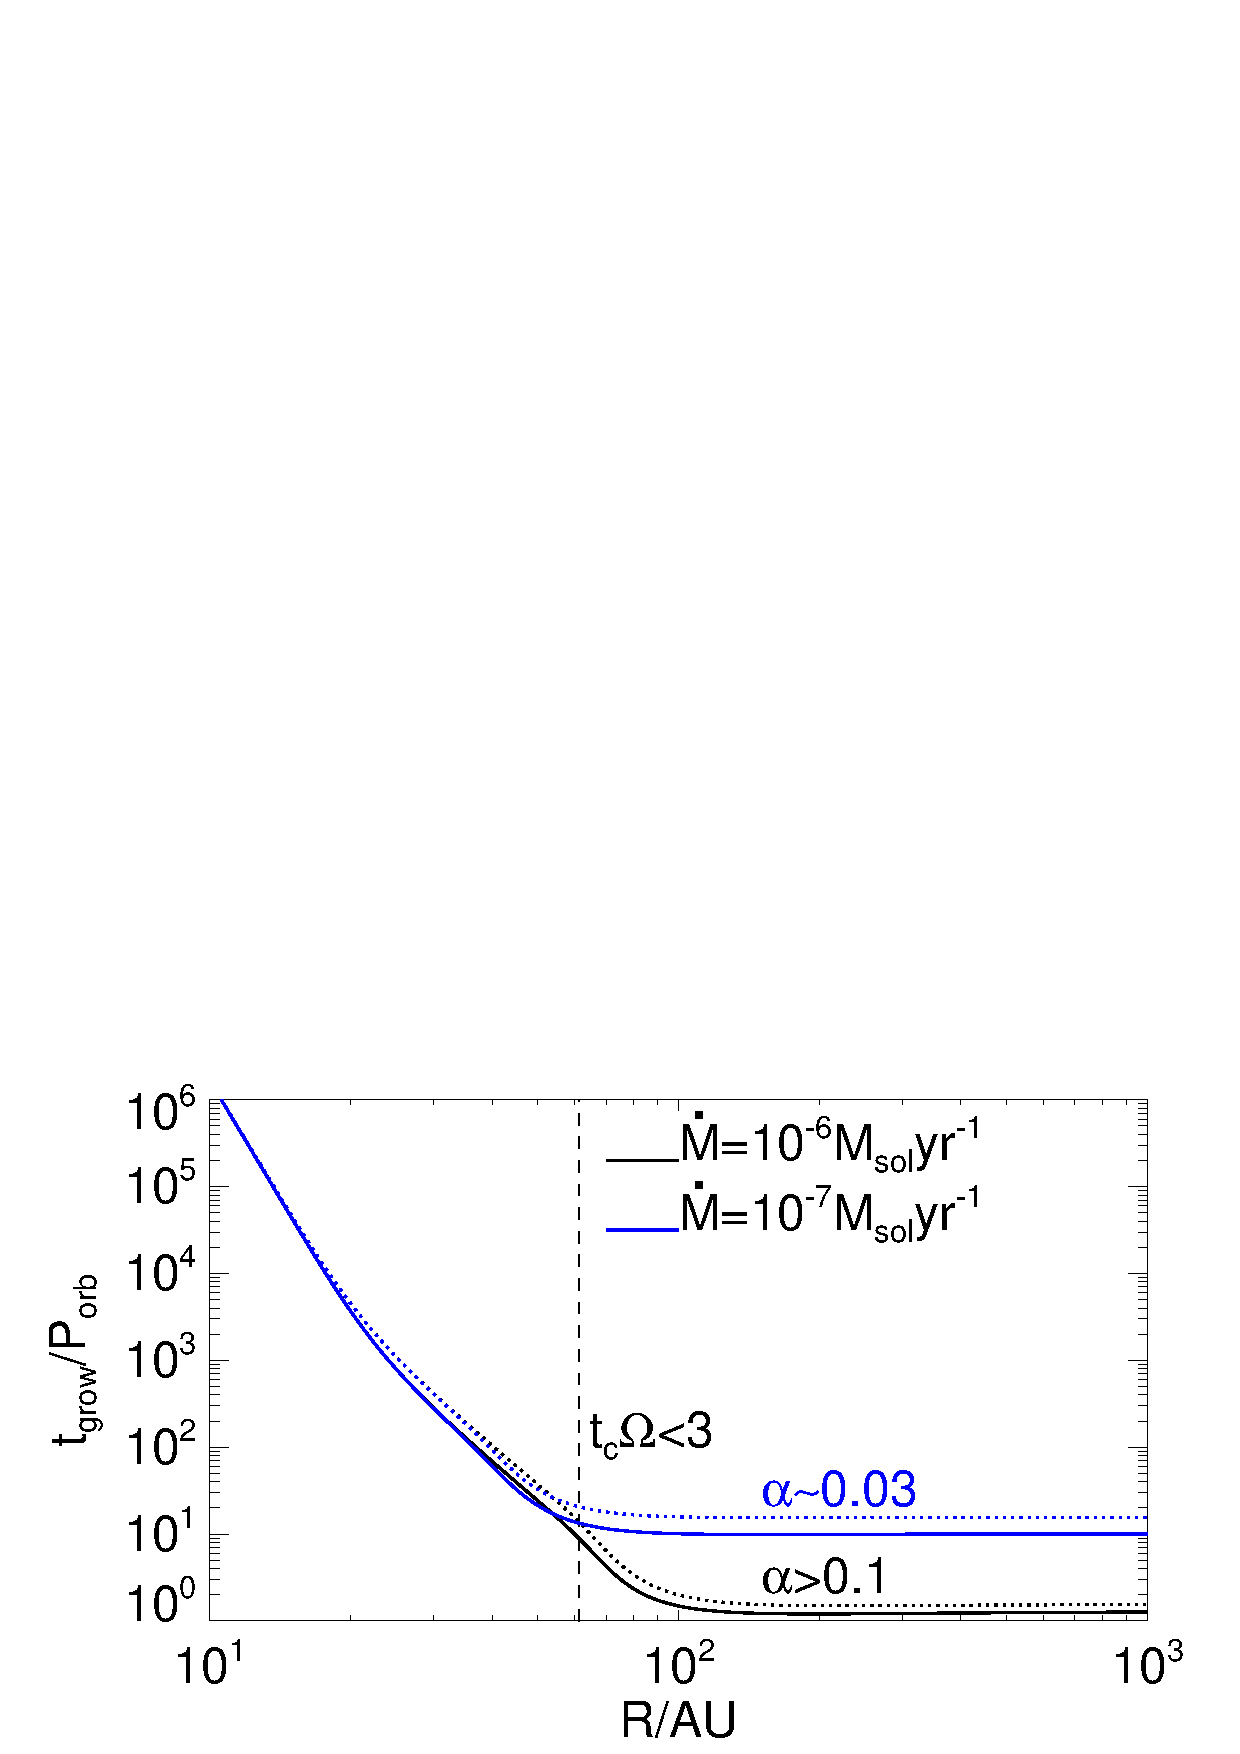
\includegraphics[width=\linewidth,clip=true,trim=0cm 1.5cm 0cm
    0.0cm]{figures/ppd_2d_growth}\\
  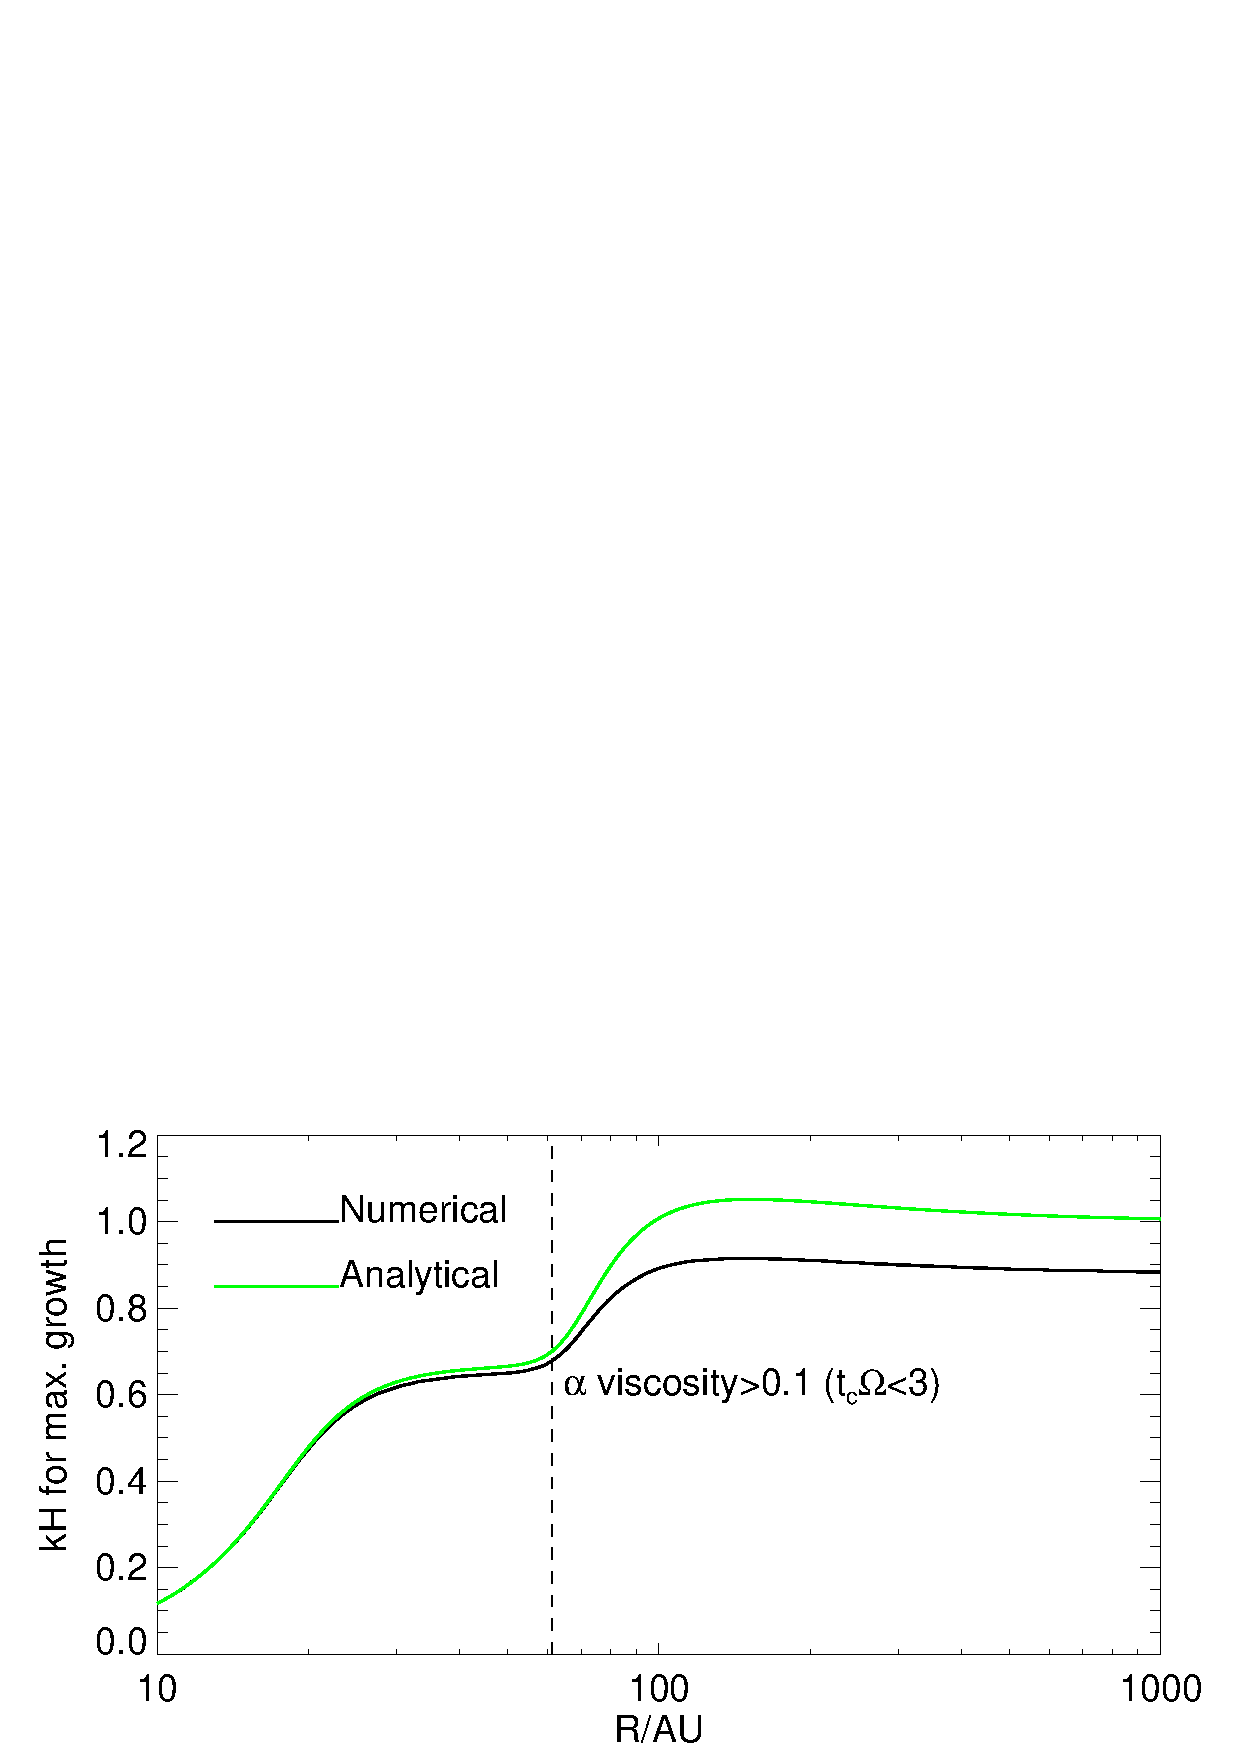
\includegraphics[width=\linewidth,clip=true,trim=0cm 0cm 0cm
    0.8cm]{figures/ppd_2d_maxk}
  \caption{Growth timescales (top) of the most unstable
    wavenumber (bottom) for viscous,
    self-gravitational modes in the 2D PPD model shown in
    Fig. \ref{rafikov_model}. 
    The black curve is obtained numerically
    from the 2D dispersion Eq. \ref{thindisk}, while green curves 
    are analytic results based on Eq. \ref{gammie_smallk}. 
    \label{rafikov_growth}}
\end{figure}


\subsection{3D PPD with radiative diffusion}
%appropriate for not-so-large distances where irrad can be neglected 
We briefly consider 3D PPDs with explicit radiative diffusion
(\S\ref{rad_cool}). 
Given the $\alpha(R)$ and $Q(R)$ profiles obtained
from the 2D model above, at each radius $R$ we obtain the vertical
structure from Eq. \ref{vert_eq1}---\ref{thermal_eq}, with 
Eq. \ref{rad_cool1}---\ref{rad_cool2} for the radiative flux.
We then solve the 3D eigenvalue problem as in \S\ref{3ddisk}, with the
additional boundary condition $\delta T^\prime(0) = \delta T(\zmax) = 0$.    
We use the same disk model as in \S\ref{pp2d_example} but 
with $T_\mathrm{irr}=0$, since our simple radiative diffusion model
does not include irradiation (\S\ref{rad_cool}). 
%physically, irrad is negligible for opt thick regions, and we are
%restricted to such regions if applying rad diff
We use a slightly smaller vertical
domain with $\rho(\zmax)=0.1\rho_0$.  %to avoid very low density 

Fig. \ref{rafikov_growth3d} show the growth rates and most unstable
wavenumber for $R\in[10,100]$AU; along with corresponding 2D 
results with softened self-gravity. There is a close match for
$R\lesssim60$AU where the disk is optically thick ($\tau\gtrsim
1$) and both models apply. However, beyond $60$AU where the disk
becomes optically-thin, radiative diffusion (the 3D curve) is not
valid and under-estimates the growth rates. %; while the $f(\tau)$
%function approximately captures opticall-thin cooling in the 2D case.  
Nevertheless, the comparison shows that the transition radius
$R_t\sim60$AU can be calculated within the 2D framework.  
%This is not surprising since the
%instability is fundamentally driven by viscous and self-gravity forces in the
%momentum equations, not the energy equation. 

\begin{figure}
  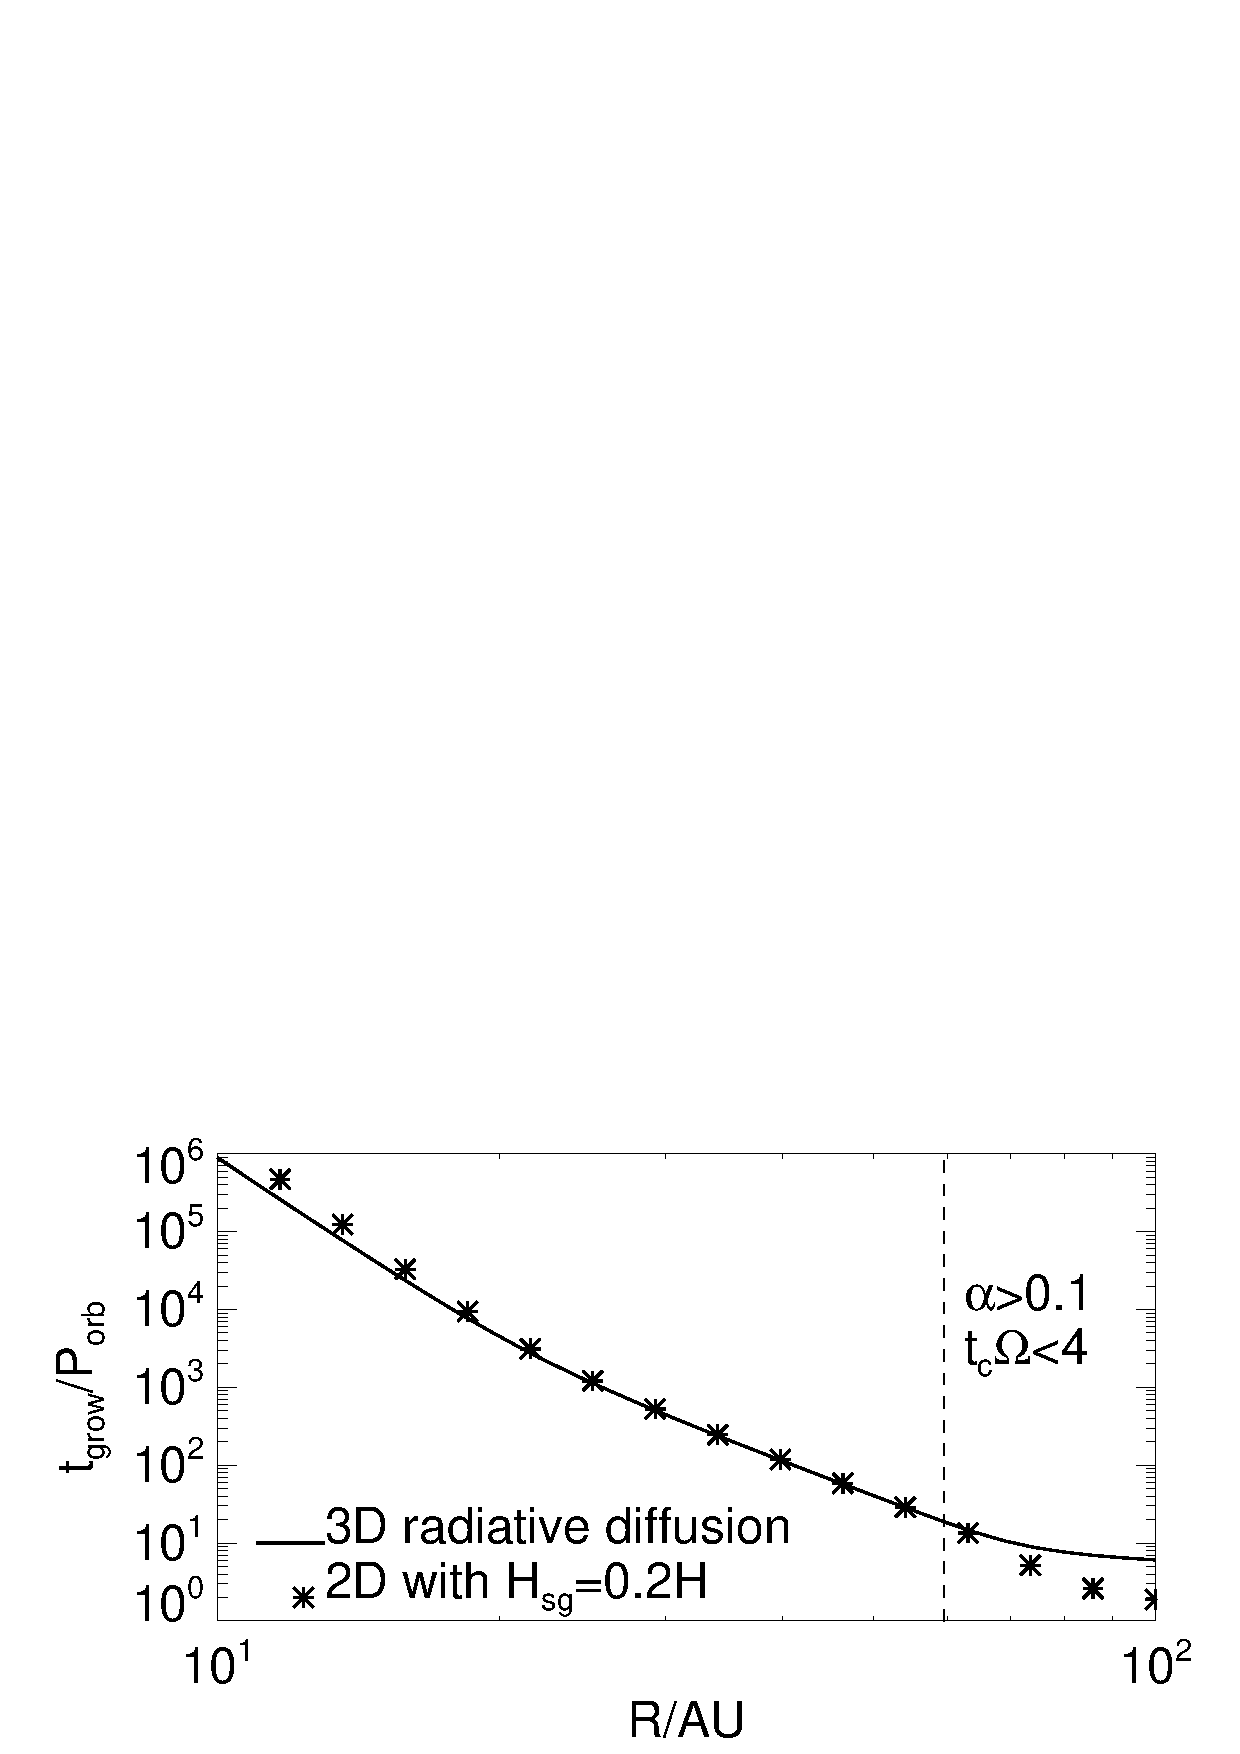
\includegraphics[width=\linewidth,clip=true,trim=0cm 1.5cm 0cm
    0.0cm]{figures/ppd_3d_rates}\\
  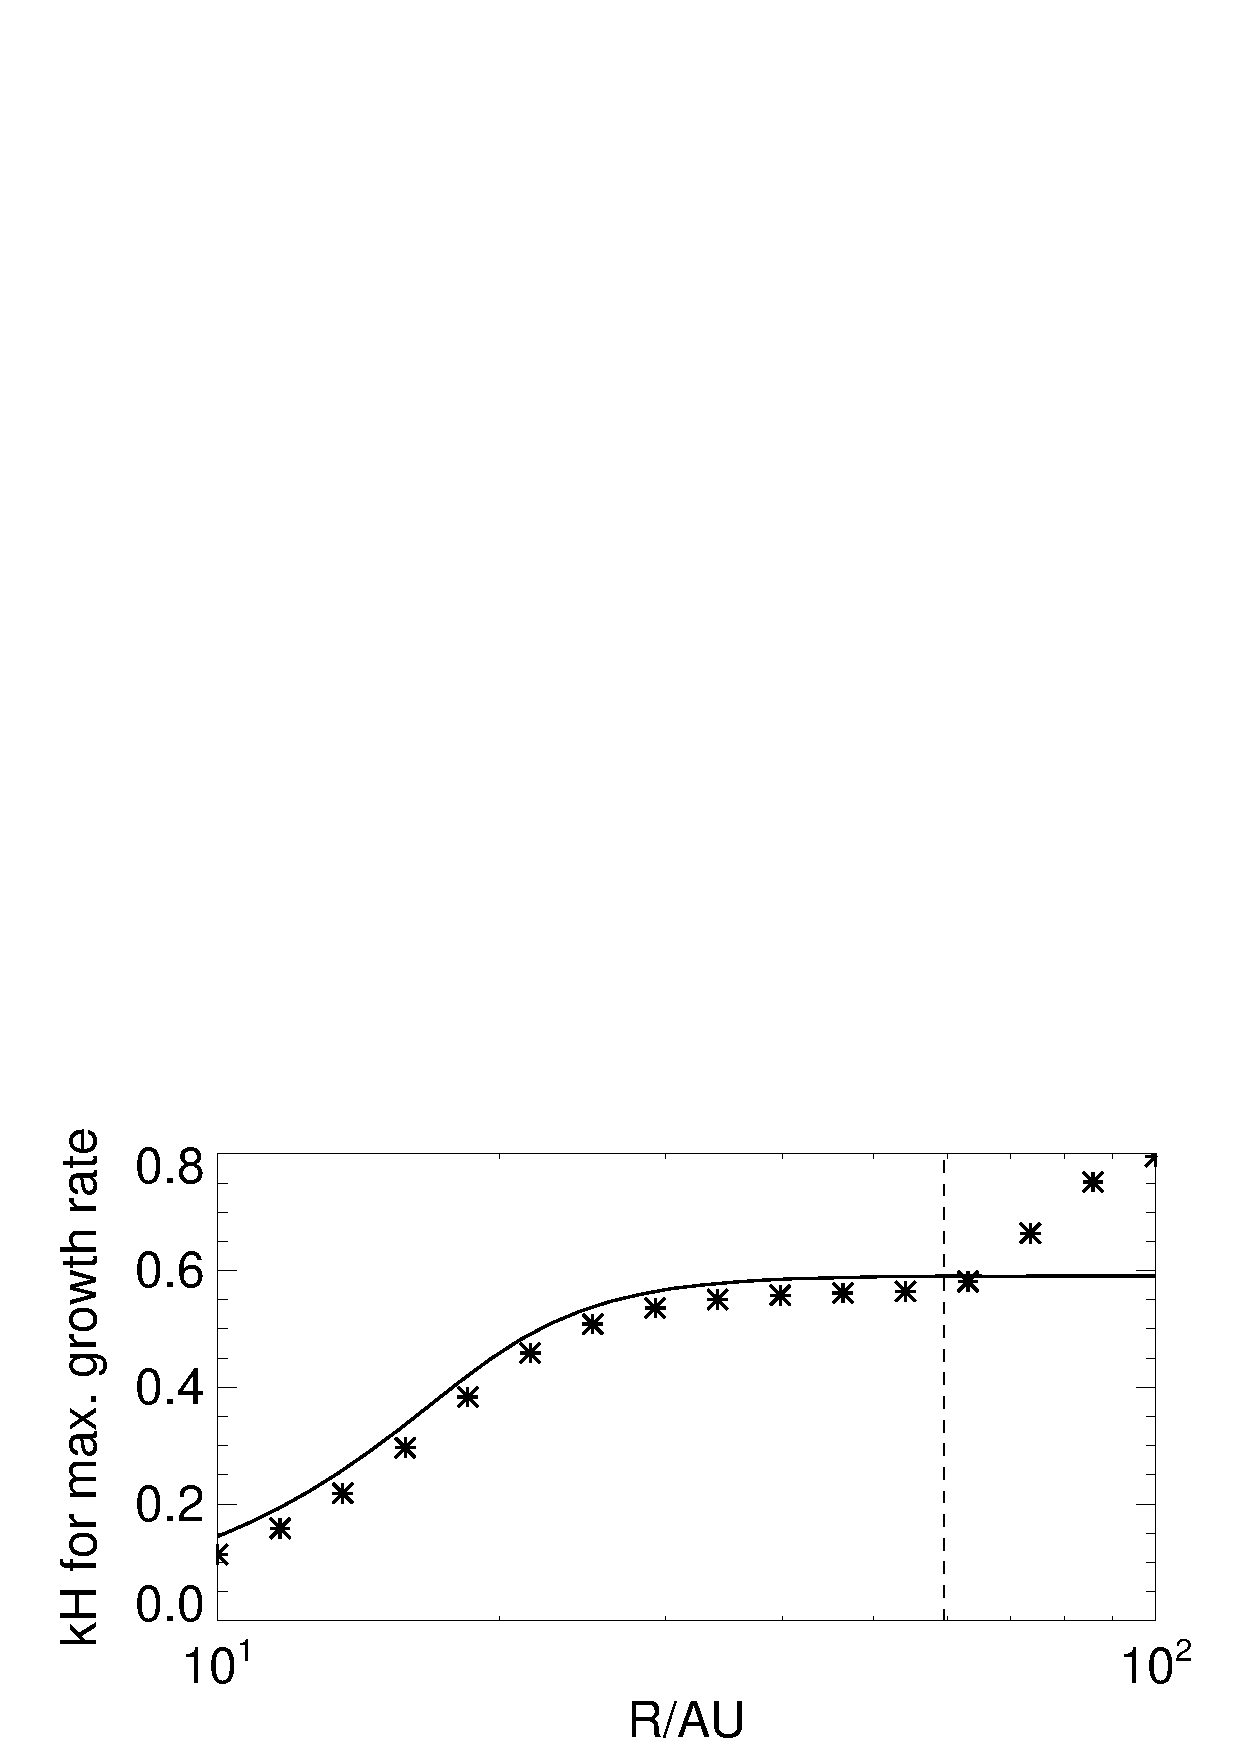
\includegraphics[width=\linewidth,clip=true,trim=0cm 0cm 0cm
    0.8cm]{figures/ppd_3d_maxk}
  \caption{Growth timescales (top) of the most unstable
    wavenumber (bottom) for viscous, 
    self-gravitating modes. The black curves are obtained
    from the 3D eigenvalue problem with radiative diffusion,
    applicable to optically-thick regions ($R\lesssim 60$AU); 
    while the green curves are obtained from the 2D corresponding
    model, which is applicable to both optically-thick and
    optically-thin regimes.  
    \label{rafikov_growth3d}}
\end{figure}



